\chapter{Análisis del problema}
{\color{blue}

Siguiendo los objetivos del proyecto \ref{sec:objetivos} se va a analizar los diferentes frameworks que existen para desarrollar una aplicación para posteriormente analizar posibles explotaciones de seguridad. \\

Como hemos visto en \ref{sec:iot}, normalmente, cuando se generan grandes datos y se transmiten a través de varios dispositivos, tiene que haber un punto específico en el que se recoja y combine todo. Este punto específico es muy esencial en una red, ya que combina todos los datos, lo que permite comprender los datos que se generan. Sin embargo, la transmisión y generación de datos sin problemas no se produce sin más. Más bien, suele ser posible gracias a un framework del Internet de las Cosas. \\

Un framework para IoT puede describirse como un ecosistema, compuesto por varios dispositivos conectados que se comunican entre sí, a través de Internet. Estos dispositivos conectados suelen funcionar para transferir y detectar datos a través de Internet, y requieren muy poca intervención humana. El framework de IoT es lo que hace posible que los dispositivos conectados tengan una comunicación fluida a través de Internet. Es un elemento tecnológico muy importante en el mundo moderno, que encuentra aplicación en casi todos los sectores. Por ejemplo, una de las principales aplicaciones del IoT es el diseño de casas inteligentes. \cite{iot-framework}\\

Es decir, un framework para IoT recoge todos principales elementos que componen el mundo del Internet de las Cosas para desarrollar una aplicación, estos elementos los podemos ver en la siguiente imagen \ref{fig:figure4}.

\begin{figure}[ht!]
    \centering
    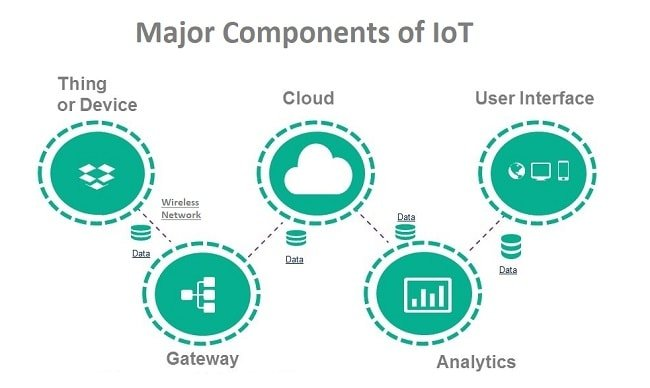
\includegraphics[width=\linewidth]{imagenes/Key-IoT-Components.jpg}
    \caption{Elementos principales de un framework en IoT. \cite{key-iot-framework}}
    \label{fig:figure4}
\end{figure}

\newpage

Cuando se esta desarrollando una aplicación, el concepto de ``framework`` se puede relacionar con otros conceptos como el de ``middleware`` y ``plataforma``. El concepto de ``plataforma`` hace referencia al lugar donde se permite desplegar y ejecutar la aplicación. Por otro lado el middleware, tiene que ver con la prestación de los servicios. Y por último, el framework se centra más en el diseño del software. Por esto, pese a que en este proyecto se va a trabajar con un framework, hay que tener en cuenta otros conceptos que rodean al desarrollo de una aplicación. \cite{nakhuva2015study}

\section{Middleware} \label{sec:middleware}

Generalmente, un middleware abstrae las complejidades del sistema o del hardware, permitiendo al desarrollador de la aplicación centrar todo su esfuerzo en la tarea a resolver, sin la distracción de preocupaciones a nivel del sistema o del hardware. Dichas complejidades pueden estar relacionadas con problemas de comunicación o de computación más generales. Un middleware proporciona una capa de software entre las aplicaciones, el sistema operativo y las capas de comunicación de la red, que facilita y coordina que facilita y coordina algún aspecto del procesamiento cooperativo. Desde el punto de vista perspectiva informática, un middleware proporciona una capa entre el software de aplicación y el software de sistema.\\

En el IoT, es probable que haya una considerable heterogeneidad tanto en las tecnologías de comunicación en uso, como en las tecnologías a nivel de sistema, y un middleware debe soportar ambas perspectivas según sea necesario. 

Basándonos en las características descritas anteriormente \ref{sec:iot} de la infraestructura del IoT y de las aplicaciones que dependen de ella, se establecen un conjunto de requisitos para que un middleware soporte el IoT. A continuación, estos requisitos se agrupan en dos conjuntos: los servicios que debe proporcionar dicho middleware y la arquitectura del sistema \cite{7322178}-\cite{7582463}.

\subsection{Requisitos del servicio de middleware}

 Los requisitos de los servicios de middleware para el IoT pueden clasificarse en funcionales y no funcionales. Los requisitos funcionales recogen los servicios o funciones, como por ejemplo abstracciones y gestión de recursos un middleware, y los requisitos no funcionales, por ejemplo fiabilidad, seguridad y disponibilidad, captan el soporte de la calidad de servicio o del rendimiento.\\
 
 En los requisitos funcionales nos encontramos:
 
 \begin{itemize}
     \item \textbf{Descubrimiento de recursos}. Ya que la infraestructura y el entorno del IoT son dinámicos, las suposiciones relacionadas con el conocimiento global y determinista de la disponibilidad de estos recursos es inviable. Pasa lo mismo con la intervención humana, es inviable que este descubra recursos. Por tanto, es importante destacar que el descubrimiento de recursos este automatizado. Cuando no hay infraestructura, el propio dispositivo debe de anunciar su presencia y los recursos que ofrece.
     \item \textbf{Gestión de recursos}. Se espera una QoS (Quality of Service) aceptable para todas las aplicaciones, y en un entorno en el que los recursos que influyen en la QoS son limitados, como el IoT, es importante que las aplicaciones cuenten con un servicio que gestione esos recursos.
     \item \textbf{Gestión de datos}. Los datos son fundamentales en las aplicaciones de IoT. En el IoT, los datos se refieren principalmente a los datos detectados o a cualquier información de infraestructura de red de interés para las aplicaciones.
     \item \textbf{Gestión de eventos}. En las aplicaciones de IoT se genera potencialmente un número masivo de eventos, que deberían gestionarse como parte integral de un middleware de IoT.
     \item \textbf{Gestión del código}. El despliegue de código en un entorno de IoT es un reto, y debe ser soportado directamente por el middleware. En particular, se necesitan servicios de asignación y de código.
 \end{itemize}
 
 En los requisitos no funcionales nos encontramos:
 
  \begin{itemize}
     \item \textbf{Escalabilidad}. Un middleware de IoT debe ser escalable para adaptarse al crecimiento de la red y las aplicaciones/servicios de IoT.
     \item \textbf{Actuación en tiempo real}. Un middleware debe proporcionar servicios en tiempo real cuando la corrección de una operación que soporta depende no sólo de su corrección lógica sino sino también del tiempo en que se realiza.
     \item \textbf{Fiabilidad}. Un middleware debe permanecer operativo durante la duración de una misión, incluso en presencia de fallos.
     \item \textbf{Disponibilidad}. Un middleware que soporte las aplicaciones de un IoT, especialmente las de misión crítica, debe estar disponible en todo momento.
     \item \textbf{Seguridad y privacidad}. La seguridad es fundamental para el funcionamiento de IoT. En el middleware de IoT, la seguridad debe tenerse en cuenta en todos los bloques funcionales y no funcionales, incluyendo la aplicación a nivel de usuario.
     \item \textbf{Facilidad de despliegue}. Hay que evitar los procedimientos complicados de instalación y configuración.
     \item \textbf{Popularidad}. Un middleware de IoT, como cualquier otra solución de software, debe recibir un apoyo y una ampliación continua.
 \end{itemize}
 
\subsection{Requisitos de arquitectura en el middleware}

En esta sección se muestran los requisitos para las abstracciones de programación y otros aspectos relacionados con la implementación.

\begin{itemize}
    \item \textbf{Abstracción de la programación}. Para el desarrollador de aplicaciones o servicios, las interfaces de programación de alto nivel deben aislar el desarrollo de las aplicaciones o los servicios de las operaciones proporcionadas por las infraestructuras subyacentes y heterogéneas del IoT. 
    \item \textbf{Interoperabilidad}. Un middleware debe funcionar con dispositivos, tecnologías y aplicaciones heterogéneas, sin esfuerzo adicional por parte del desarrollador de aplicaciones o servicios.
    \item \textbf{Basado en el servicio}. Una arquitectura de middleware debe estar basada en servicios para ofrecer una gran flexibilidad cuando sea necesario añadir funciones nuevas y avanzadas al middleware de un IoT.
    \item \textbf{Adaptable}. Un middleware debe ser adaptativo para poder evolucionar y adaptarse a los cambios de su entorno.
    \item \textbf{Consciente del contexto}. El conocimiento del contexto es un requisito clave en la construcción de sistemas adaptativos y también en el establecimiento de valor de los datos recogidos.
    \item \textbf{Autónomo}. Los dispositivos, tecnologías y aplicaciones son participantes activos en los procesos del IoT y deben estar habilitados para interactuar y comunicarse entre sí sin la intervención intervención humana.
    \item \textbf{Distribuido}.  Las aplicaciones de un sistema IoT a gran escala de un sistema IoT intercambian información y colaboran entre sí.
\end{itemize}


\section{Frameworks IoT}

Una vez hemos visto requisitos que necesitamos en nuestro middleware, se van a comentar una serie de requisitos que buscamos en nuestro framework IoT. \cite{agarwal2020investigating}-\cite{dumitru2017iot}-\cite{nakhuva2015study}

\subsection{Requisitos para seleccionar un framework IoT} \label{requisitosFramework}

Algunos requisitos principales en los que nos tenemos que fijar a la hora de seleccionar un entorno de desarrollo son:

\begin{itemize}
    \item \textbf{Seguridad y privacidad}. El framework debe de proporcionar seguridad en la capa de transporte para conexiones seguras (encriptación SSL) y no comprometer en el entorno de trabajo. Con esto, conseguimos privacidad, autenticación e integridad en los datos. 
    \item \textbf{Dificultad de uso}. Seleccionar un framework que sea sencillo de usar para desarrolladores. Esto incluye el lenguaje de programación que se use para hacer la aplicación.
    \item \textbf{Código abierto}. Se trata de evitar aquellos framework en los que hay que pagar por su uso o que den un periodo de prueba gratuito. Las plataformas de código abierto permiten que las plataformas sean gestionadas por el desarrollador según sus necesidades.
    \item \textbf{Soporte}. Se busca un framework que sea popular y tenga un equipo y comunidad activa, que continuamente este aportando nuevas características al proyecto.
\end{itemize}

También existen otras características en las que nos podemos fijar que pueden resultar útiles dependiendo del tipo de aplicación que queremos desarrollar:

\begin{itemize}
    \item \textbf{Tipo de soporte de protocolo de comunicación}. Los dispositivos IoT soportan múltiples protocolos de comunicación. Algunos son ligeros y otros son seguros. El protocolo a elegir depende de los requisitos de la aplicación IoT. CoAP es similar a HTTP pero es ligero, por lo que es más adecuado para aplicaciones móviles. MQTT también es ligero y soporta el concepto de broker, por lo que es bueno para aplicaciones de ancho de banda limitado. CoAP es bueno para la multidifusión y la difusión.
    \item \textbf{Disponibilidad}. La disponibilidad y la estabilidad son parámetros importantes para los requisitos del IoT. Por ejemplo, una aplicación enfocada a la salud requiere que los datos datos médicos del paciente para ser monitorizados continuamente.
    \item \textbf{Tecnologías de almacenamiento utilizadas}. Diferentes tecnologías de almacenamiento y procesamiento sobre la nube soportan diferentes tipos de análisis. Según los requisitos de procesamiento de datos, se puede seleccionar una nube con diferentes tecnologías de almacenamiento.
    \item \textbf{Tipo de análisis soportado}. Las aplicaciones de IoT suelen requerir datos en tiempo real o datos históricos para el desarrollo de la aplicación. La elección de la tecnología adecuada para aplicar la analítica al tipo de datos generados por el dispositivo en la aplicación es otro factor importante.
\end{itemize}

\subsection{Varios framework IoT}

\subsubsection{KAA IoT}
    Es totalmente gratis, tiene capacidad para gestionar millones de sensores, recoger y analizar datos en tiempo real y visualizarlos, gestionar y conectar productos inteligentes con ayuda de nube. Permite la gestión de los datos de los objetos conectados y la infraestructura de back-end que proporciona los componentes del SDK del servidor y del endpoint. KAA proporciona la funcionalidad de back-end necesaria para operar una solución IoT. Proporciona flexibilidad a los usuarios para implementar sus propias políticas de seguridad.\\ 
    
    Kaa proporciona un gateway que aporta la posibilidad de conectar diferentes redes entre si. Los protocolos de comunicación que usa para comunicarse con los dispositivos son MQTT y COAP. Para especificar un dispositivo se hace en JSON, donde cada dispositivo es un objeto. Kaa permite el análisis de datos y para ello usa tecnologías como NoSQL, Cassandra, Hadoop y MongoDB. Kaa soporta lenguajes de programación como Java, C, C++. \cite{kaaiot}
    
\subsubsection{ThingSpeak}

Es un framework que se caracteriza por sus visualizaciones y predicciones utilizando MATLAB. Soporta datos con formato JSON y XML. Es de código abierto. Soporta múltiples dispositivos y permite utilizar protocolos como MQTT o Rest API para la comunicación entre dispositivos. Proporciona seguridad en la capa de transporta con encriptación en las comunicaciones. \cite{thingspeak}

\subsubsection{Macchina.io}

Este framework se divide en dos productos, el primero es el \textbf{Edge} que permite que las aplicaciones se ejecuten en dispositivos basados en Linux utilizando C++ y Javascript. Y el segundo producto es el \textbf{Remote} que permite gestionar la infraestructura mediante paneles web y aplicaciones móviles. Una de las tecnologías que utiliza es SQLite e incluye soporte para protocolos de comunicación como MQTT, SOAP, HTTP. \cite{macchinaio}
 
\subsubsection{Altair (Carriots)}

Altair, anteriormente ``Carriots``, es una plataforma diseñada para proyectos IoT. Permite integrar los dispositivos de IoT a una aplicación externa que requiera de los datos mientras ellos se encargan del almacenamiento y la comunicación. Soporta XML, JSON y API Rest. No es gratis, tiene un plan de subscripción. Permite escribir aplicaciones en Java. Para la comunicación entre dispositivos usa MQTT, no posee encriptación en la comunicación pero si posee un mecanismo de autenticación y autorización. Para el almacenamiento usa NoSQL. \cite{altair}

\subsubsection{Zetta}

Es una plataforma de código abierto construida sobre Node.js para crear servidores del Internet de las Cosas que se ejecutan a través de ordenadores geodistribuidos y la nube. Zetta combina las API de REST, los WebSockets y la programación reactiva, lo que resulta perfecto para ensamblar muchos dispositivos en aplicaciones de uso intensivo de datos en tiempo real. Zetta tiene la capacidad de convertir cualquier dispositivo en una API. Al comunicarse con microcontroladores como Arduino y Spark Core, Zetta puede proporcionar a cada dispositivo una API REST tanto localmente como en la nube. Zetta es ``developer friendly`` lo que significa que es sencillo desarrollar usando esta plataforma. Entre las tecnologías que usa esta API Rest y JSON. \cite{zetta}

\subsubsection{Temboo}

Es un framework que entra dentro de la categoría de plataformas que son ``developer friendly``, es decir, para conectar dispositivos y hacer tareas simples se hace de manera rápida y sin complicaciones en el código. Soporta datos en Excel, CSV, XML y JSON. Soporta lenguajes de programación como C, Java, Python y Javascript. No es gratuito, requiere de un plan de subscripción para empezar a utilizarlo. Tiene soporte con múltiples dispositivos, entre ellos Arduino y a destacar Samsung Artik. Los protocolos que soporta son HTTP, MQTT, CoAP. Y tiene soporte de tecnologías como Microsoft Power BI y Google BigQuery. \cite{temboo}

\subsubsection{Particle}

Particle es una plataforma de IoT escalable, fiable y segura. Una característica clave es la capacidad de ejecutar código de cableado de Arduino y Raspberry Pi haciendo más fácil conectar componentes electrónicos a la nube. Los primeros 100 dispositivos que se conecten son gratuitos. En cuanto a la seguridad, es uno de los frameworks con más características relacionadas con esta, posee encriptación en las comunicaciones, autenticación, autorización y posibilidad de auditoría de seguridad, todo esto bajo el protocolo HTTP. Soporta datos en formato CSV y se puede desarrollar código Javascript y en particle js, una librería ligera de Javascript.

\subsubsection{Soluciones comerciales}

Hay otras soluciones comerciales donde nos encotramos plataformas como AWS IoT, Microsoft Azure IoT Hub, IBM Watson IoT, Google IoT y Oracle IoT. Todas estas alternativas son bastante similares a todas las comentadas hasta el momento, se diferencian entre si por ciertas características como el soporte en lenguajes de programación, donde aparecen lenguajes que no vemos en otras plataformas como son Ruby, .NET, Go, php. En la siguiente tabla se muestran características de estas plataformas : 


\begin{table}[H]
	\centering
	\label{tabla-commercial-solutions}
	\resizebox{\textwidth}{!}{%
	\begin{tabular}{ | m{3.5cm} | m{2cm} | m{3cm} | m{2cm} | m{3cm} |}
		\toprule
		\rowcolor[HTML]{ECF4FF} 
		\textbf{Framework IoT} & \textbf{Soporte de datos} & \textbf{Soporte de lenguajes de programación} & \textbf{Protocolos} & \textbf{Seguridad} \\ \midrule
		\cellcolor[HTML]{ECF4FF}\textbf{\begin{tabular}[c]{@{}c@{}}AWS IoT\end{tabular}} & JSON                & Java, C, NodeJS, Javascript, Python, iOS, Android & HTTP, MQTT, Websockets & Encriptación, autenticación, autorización, auditoría                  \\
		\cellcolor[HTML]{ECF4FF}\textbf{\begin{tabular}[c]{@{}c@{}}Microsoft Azure IoT\end{tabular}} & JSON  & .NET, UWP, Java, C, NodeJS, Ruby, Android, iOS & HTTP, AMQP & Encriptación, autenticación, autorización, políticas definidas por usuario                   \\
		\cellcolor[HTML]{ECF4FF}\textbf{\begin{tabular}[c]{@{}c@{}}IBM Watson IoT\end{tabular}} & JSON, CSV  & C\#, C, Python, Java, NodeJS & MQTT & Autenticación, Autorización                  \\
		\cellcolor[HTML]{ECF4FF}\textbf{\begin{tabular}[c]{@{}c@{}}Oracle IoT\end{tabular}} & JSON, CSV  & Java, Javascript, Android, C, iOS & REST API & Autenticación, Autorización \\
		\cellcolor[HTML]{ECF4FF}\textbf{\begin{tabular}[c]{@{}c@{}}Google IoT\end{tabular}} & JSON                & Go,Java, .NET, Node.js, php, Python, Ruby & MQTT, HTTP & Autenticación                  \\ \bottomrule
	\end{tabular}}
	\caption{Características de soluciones comerciales para framework IoT. \cite{agarwal2020investigating}}
\end{table}

\section{Elección del framework} \label{eleccion-framework}

Como framework para desarrollar la aplicación se ha optado por trabajar con \textbf{Kaa IoT}. La motivación de su uso viene de cumplir todos los requisitos establecidos en la sección \ref{requisitosFramework}.

\begin{itemize}
    \item \textbf{Seguridad y privacidad}. Kaa IoT proporciona autenticación del cliente con certificado SSL/TLS, por tanto, todas sus comunicaciones van a estar cifradas. Aparte, para el proyecto puede resultar útil posible implementación de nuestras propias políticas de seguridad.
    \item \textbf{Dificultad de uso}. No llega a ser un framework ``developer friendly``, pero en la documentación del framework \cite{kaaiot} hay varios tutoriales como para desarrollar sin mucha dificultad una aplicación , explicando en cada apartado las palabras clave o conceptos que se necesitan para entender todo lo que se esta haciendo en la construcción de la aplicación. Aquellos frameworks ``developer friendly``, por el hecho de ser plataformas donde ofrecen ayudar por desarrollar y desplegar la aplicación requieren de una subscripción para hacer uso de estas.
    \item \textbf{Código abierto}. Es un framework gratuito, evitamos todos los frameworks que requieren de un plan de subscripción.
    \item \textbf{Soporte}. Es de los frameworks más conocidos. Y tienen una comunidad activa, esto se puede observar en su repositorio de github \footnote{Enlace a repositorio de Kaa IoT: https://github.com/kaaproject/kaa}, que cada poco tiempo van añadiendo nuevas características y documentación al proyecto.
\end{itemize}


Otra elección interesante podría haber sido \textbf{macchina.io} no cumple con el requisito de dificultad de uso. En comparación con \textbf{Kaa IoT}, macchina.io no dispone de tanta documentación como el framework seleccionado.


\section{Explotación de vulnerabilidad} \label{exploit-analysis}

Para empezar, ya que vamos a trabajar con MQTT vamos a analizar este protocolo de comunicación para posteriormente atacarlo para así explotar una vulnerabilidad de nuestra aplicación. Una vez visto como funciona MQTT, veremos las etapas de un ataque y las herramientas que necesitamos en cada una de las etapas.

\subsection{MQTT en profundidad}

Ya se habló de este protocolo en \ref{protocolos}. Cada protocolo IoT requiere diferentes vectores de ataque. MQTT no es, por defecto, seguro, y muchos despliegues de MQTT parecen haberse saltado la letra pequeña cuando se trata de usar MQTT de forma segura. Así que vamos a explotarlo. \\

La definición oficial de MQTT viene de \textbf{mqtt.org} \cite{mqtt}: \\

\textit{``MQTT son las siglas de MQ Telemetry Transport. Se trata de un protocolo de publicación/suscripción, extremadamente sencillo y ligero, diseñado para dispositivos limitados y redes de bajo ancho de banda, alta latencia o poco fiables. Los principios de diseño consisten en minimizar el ancho de banda de la red y los requisitos de recursos de los dispositivos, al tiempo que se intenta garantizar la fiabilidad y cierto grado de seguridad en la entrega. Estos principios también hacen que el protocolo sea ideal para el emergente mundo de los dispositivos conectados "máquina a máquina" (M2M) o "Internet de las cosas", y para aplicaciones móviles en las que el ancho de banda y la energía de la batería son muy importantes. ``} \\


MQTT es un protocolo de publicación/suscripción que permite la comunicación de uno a muchos a través de un broker MQTT. Poder comunicarse con todos los dispositivos conectados al broker facilita los ataques activos a gran escala. Un atacante que sea capaz de espiar y saber qué tipo de mensajes se están enviando a través del broker puede utilizar posteriormente esta información para atacar simultáneamente a todos los dispositivos conectados a él. \\

Tiene una característica llamada suscripción con comodines, y muchos usuarios de MQTT pasan por alto las implicaciones de esto en la seguridad. Un despliegue por defecto de MQTT sin autorización permite a cualquier cliente conectado suscribirse a todos los mensajes, y un atacante puede utilizar esta información para conocer y registrar todos los mensajes intercambiados en una solución IoT. Por esto, es bastante factible realizar un ataque de escalado de privilegios. \cite{mqtt-security-1} \\


\subsection{Características de MQTT}

\begin{itemize}
    \item Patrón de publicación y suscripción.
    \item Formatos de paquetes simples: cargas útiles binarias.
    \item Version actual: 3.1.1 (Dec/2015).
    \item El protocolo se ejecuta a través de TCP.
    \item Puerto por defecto: 1883/TCP (no encriptado).
\end{itemize}


El modelo de \textbf{publicación/suscripción} se compone de:

\begin{itemize}
    \item \textbf{Editor,} publica un mensaje en uno (o varios) temas del broker.
    \item \textbf{Broker,} dirige todos los mensajes de los editores a los suscriptores.
    \item \textbf{Tema,} consta de uno o varios niveles separados por una barra diagonal (por ejemplo, /smartshouse/livingroom/temperature).
\end{itemize}

\begin{figure}[hb!]
    \centering
    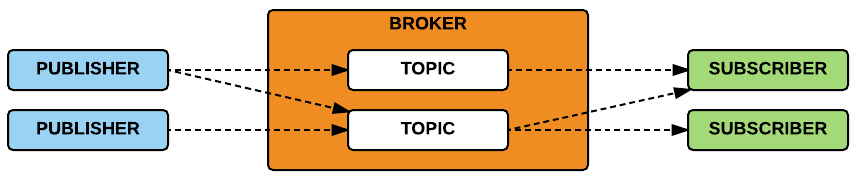
\includegraphics[width=\linewidth]{imagenes/sub-pattern-mqtt.png}
    \caption{Modelo publicación/suscripción \cite{disenio-mqtt}}
    \label{fig:figure13-mqtt-analysis}
\end{figure}

\subsection{Seguridad en MQTT}

La nota oficial de MQTT acerca de la seguridad de este (\textbf{mqtt.org}) \cite{mqtt}: \\

\textit{``Puedes pasar un nombre de usuario y una contraseña con un paquete MQTT en la V3.1 del protocolo. La encriptación a través de la red puede ser manejada con SSL, independientemente del protocolo MQTT en sí mismo (vale la pena señalar que SSL no es el más ligero de los protocolos, y añade una sobrecarga de red significativa). Se puede añadir seguridad adicional mediante una aplicación que cifre los datos que envía y recibe, pero esto no es algo integrado en el protocolo, con el fin de mantenerlo simple y ligero.``}\\

Aquí tenemos dos puntos a considerar:

\begin{enumerate}
    \item La autenticación es totalmente opcional
    \item Si se realiza la autenticación, el cifrado no se utiliza por defecto (las credenciales se envían en texto claro). Los ataques MITM aún pueden ser ejecutados para robar contraseñas.
\end{enumerate}

\subsection{Fases de un ataque}

Para poder contrarrestar un ataque debemos conocer las fases de este, por esto vamos a hacer un \textbf{test de intrusión} o \textbf{Pentest}. Esto es una prueba de seguridad ofensiva que simula un ataque real en un entorno controlado. El objetivo principal de este tipo de pruebas es identificar las posibles brechas en la seguridad de un sistema de manera que, al simular el comportamiento de los atacantes reales, podamos descubrir vulnerabilidades y agujeros de seguridad que necesiten ser corregidos para que no sean explotados por parte de atacantes reales. \cite{pentesting} \\

Las fases y tecnologías dentro de cada fase que nos encontramos son:

\begin{enumerate}
    \item \textbf{Reconocimiento}, se recolecta información del sistema de forma activa o pasiva. En este caso se van a usar herramientas como nmap o netstat para recopilar información de dominios, IPs, puertos y servicios.
    \item \textbf{Análisis de vulnerabilidades}, aquí se analizará la información recopilada de la fase de reconocimiento. Se puede investigar por internet posibles vulnerabilidad, por ello se puede mencionar a \textbf{CVE} \footnote{https://cve.report/vendor/mqtt}, para conocer posibles vulnerabilidad.
    \item \textbf{Explotación}, en esta fase se realizan las acciones necesarias para poder comprometer al sistema, los usuarios o la información que se maneja. Para este proyecto se usará \textbf{Metasploit}, es una herramienta que proporciona información acerca de vulnerabilidades de seguridad y ayuda en test de penetración.
\end{enumerate}

}